\documentclass[a4paper,12pt]{article}
\usepackage{jheppub}
\usepackage{taro}

\title{Mathematical Methods in Physics}

\author[a]{Taro V. Brown}

\affiliation[a]{Department of Physics, UC Davis, One Shields Avenue, Davis, CA 95616, USA }


% e-mail addresses: one for each author, in the same order as the authors
\emailAdd{taro.brown@nbi.ku.dk}


\abstract{}
\begin{document} 
\maketitle
\flushbottom
\tableofcontents
\newpage
\section{Residue Calculus}
If $f(z)$ has a pole of order $m$ at $z=a$, thrn
\begin{equation}
\Res[f(z=a)]=\frac{1}{(m-1)!}\lim_{z\to a}\dv[m-1]{}{z}[(z-a)^mf(z)]
\end{equation}
Residue theorem:
If you have some domain with poles in them, you can pinch the conbtour of integration (since it doesn't affect the end results) around these poles. $f$ is analytic in the domain and on the boundary then
\begin{equation}
\oint _C \dd z  f(z)=2\pi i \sum_{a_i\in D}\Res[f(a_i)]\end{equation}
\underline{Jordan's Lemma:} Integrals along the real line, so the contour is just the real axis, so it is open:
\begin{equation}
	\sum_{-\infty}^{\infty}f(x)\dd x= \lim_{R\to \infty }\int_{-R}^{R}f(x)\dd x
\end{equation}
to convert this to a contour integral we have to close the open segment. This can be done by making a semi circle in either the upper or the lower half-plane.
\\
Jordan's Lemma says:
Let $C_R$ be a semicircle of radius R in e.g. upper half plane (UHP) and f is analytic in UHP and decays faster than $|z|^{-1}$ for $\arg(z)\in [0,\pi]$\footnote{This argument just specifies the UHP}, then
\begin{equation}
	\int_{C_R} \dd z e^{i\alpha z}\to 0 \text{ as } R\to \infty, \text{ for } \alpha > 0
\end{equation}
This gets an exponential damping through $i\alpha z=i\alpha \Re (z)-\alpha \Im(z)$, so the integral is bounded by $1/R$ which goes to zero when we take $R\to \infty$\\
\underline{Example:}
Rational functions
\begin{equation}
\int_{-\infty}^{\infty}\frac{p(x)}{q(x)}
\end{equation}
with $p$ and $q$ begin polynomials with $q$ being one degree higher than $p$, also assume $q$ doesn't have a zero along the real line. We can the write using J's Lemma
\begin{equation}
	\int_{-\infty}^{\infty}\frac{p(x)}{q(x)}=\lim_{R\to \infty}\int_{-R}^{R}\frac{p(x)}{q(x)}\to \oint_\gamma \dd z\frac{p(z)}{q(z)}=2\pi i \sum_{a_i\in\text{UHP}}\Res[\frac{p(a_i)}{q(a_i)}]
\end{equation}
where $\gamma$ is closed contour in either UHP or LHP with LHP giving a negative sign.\\
\underline{Example I}
\begin{equation}
\begin{aligned}
\int_{0}^{\infty}\frac{x^2}{(x^2+1)(x^2+9)}&=\frac{1}{2}\int_{-\infty}^{\infty}\frac{x^2}{(x^2+1)(x^2+9)}\\
&\to \frac{1}{2}\oint_\gamma \dd z \frac{z^2}{(z^2+1)(z^2+9)}
\end{aligned}
\end{equation}
This has zeros at $z^2=1$ and $z^2=9$ so 4 simple poles at $z=\{-3i,-i,i,3i\}$. We then include the residues at these poles, so
\begin{equation}
\begin{aligned}
	&\int_{0}^{\infty}\frac{x^2}{(x^2+1)(x^2+9)}\\
	&=\frac{1}{2}2\pi i \left\{
	\Res[\frac{z^2}{(z-i)(z+i)(z+3i)(z-3i)}]_{z=i}+	\Res[\frac{z^2}{(z-i)(z+i)(z+3i)(z-3i)}]_{z=3i}
	\right\}\\
	&=\frac{1}{2}2\pi i \left\{[\frac{z^2}{(z+i)(z+3i)(z-3i)}]_{z=i}+	[\frac{z^2}{(z-i)(z+i)(z+3i)}]_{z=3i}
	\right\}\\
	&=\frac{1}{2}2\pi i \left\{\frac{i^2}{(2i)(4i)(2i)}+\frac{(3i)^2}{(3i-i)(3i+i)(3i+3i)}]
	\right\}
\end{aligned}
\end{equation}
For simple pole one can just drop the pole part and evaluate the remainder at the pole to get the residue.\\
\underline{Example II}
Sin for imaginary values is just Sinh, so $\sin(a z)\to 0$ as $Im(z)\to \pm\infty$ depending on sign of $a:\pm$. Using $\sin(az)=\Im(e^{iz})$
\begin{equation}
	\begin{aligned}
		\int_{0}^{\infty}\frac{x \sin(a x)}{(x^4+4)}&=\Im \oint_\gamma \frac{z e^{iaz}}{(x^4+4)}
	\end{aligned}
\end{equation}
This has poles at $z=\pm 1 \pm i$ so
\begin{equation}
	\begin{aligned}
		\int_{0}^{\infty}\frac{x \sin(a x)}{(x^4+4)}&=\Im \oint_\gamma \frac{z e^{iaz}}{(x^4+4)}
	\end{aligned}
\end{equation}
...\\
...\\
\underline{Example III}
Functions of trig functions
\begin{equation}
	\begin{aligned}
		\int_{0}^{2\pi} \dd \theta F(\sin \theta, \cos \theta )
	\end{aligned}
\end{equation}
with $\sin\theta = \frac{z-\frac{1}{z}}{2}$ $\cos\theta = \frac{z+\frac{1}{z}}{2}$ and $\dd \theta=\frac{\dd z}{iz}$, so
\begin{equation}
	\begin{aligned}
		I=\oint_{|z|=1} \frac{\dd z}{iz} F(\frac{z-\frac{1}{z}}{2}, \frac{z+\frac{1}{z}}{2} )
	\end{aligned}
\end{equation}
E.g.
\begin{equation}
	\begin{aligned}
		\int_{0}^{2\pi} \dd \theta \frac{1}{1+a\cos \theta}\\
		&=\frac{2}{i}\oint_{|z|=1} \frac{\dd z}{iz\left[1+a\frac{z^2+1}{2z}\right]}\\
		&=\oint_{|z|=1} \frac{\dd z}{az^2+2z+a}\\
		&=\frac{2\pi}{\sqrt{1-a^2}}
	\end{aligned}
\end{equation}
the poles are at $z=-\frac{-1\pm\sqrt{1-a^2}}{a}$\\
\underline{Principal Value Prescription (Feynman $i\epsilon$ prescription)}
If one tries to integrate a function that blows up on the real line, e.g.
\begin{equation}
\int_{-\infty}^{\infty}\frac{f(x)}{x-a}, ~~~ a\in \mathds{R}
\end{equation}
The way to integrate this is by jumping the pole on axis either below or above, so the integral is slit into
\begin{equation}
	\int_{-\infty}^{a-\epsilon}\frac{f(x)}{x-a}+\int_{a+\epsilon}^{\infty}\frac{f(x)}{x-a}+\int_\Gamma\frac{f(x)}{x-a}
\end{equation}
with $\Gamma$ the contour around the pole on the axis. Then when closing the contour using Jordan's lemma, we have to close it in the plane opposite of the the one we jumped the pole in.
The integral then gives
\begin{equation}
I = P\mp i \pi f(a)
\end{equation}
where P is the principal part (the part of the integral that ignores the divergent pole at $a$). In Feynmans language:
\begin{equation}
\frac{1}{x-a\pm i\epsilon}=P(\frac{1}{x-a})\mp i \pi\delta(x-a)
\end{equation}
\underline{Example I}\\\\
Using the Feynman Prescription
\begin{equation}
\begin{aligned}
 \int_{0}^{\infty} \dd x\frac{\sin x}{x} &=\frac{1}{2}\Im\left[ \int_{-\infty}^{\infty} \dd x\frac{e^{ix}}{x}\right]\\
 &=\frac{1}{2}\Im\left[ \int_{-\infty}^{\infty} \dd x\frac{e^{ix}}{x-i\epsilon}\right]\\
  &=\frac{1}{2}\Im\left[P \int_{-\infty}^{\infty} \dd x\frac{e^{ix}}{x-i\epsilon}+i\pi \int_{-\infty}^{\infty} \dd x e^{ix}\delta(x)\right]\\
  &=\pi/2
\end{aligned}
\end{equation}
\underline{Example II}
\begin{equation}
	\begin{aligned}
		\int_{0}^{\infty} \dd k\frac{e^{ikx}}{k^2-m^2} &=\frac{1}{2}\Im\left[ \int_{-\infty}^{\infty} \dd x\frac{e^{ix}}{x}\right]
		&=-\frac{\pi}{x}\sin(m|x|)
	\end{aligned}
\end{equation}
Often the principal is real and since we take the imaginary part, the only contribution comes from the pole 
\section{Conformal Mapping}
Very useful tool in fluid dynamics, since it is very closely tied to solving the Laplace equation in two dimensions.\\
We have seen that if $f$ is analytic then $\Re(f)$ and $\Im (f)$ are harmonic, i.e. they satisfy Laplace's equations in $d=2$ automatically from Causchy-Riemann.
\\\\
\begin{equation}
z\to f(z)
\end{equation}
we can think of this map from some domain in z-plane to $w=f(z)$. It maps points to points. So if $f$ is analytic in the first region\footnote{We only consider simply connected domains, i.e. no holes in the domains.} then it is analytic after the map.
\\\\
\underline{Riemann Mapping Theorem}
The interior of any domain $\Omega$ (with more than 1 point on $\partial\Omega$), can be conformally mapped to the unit disc $D$ with the boundary being mapped to the unit circle. The map can be made unique by choosing to map a particular point $w_0\in \Omega$ to the origin of $D$ and by orienting a particular directions from $w_0$ to the real axis in $D$.
% TODO: \usepackage{graphicx} required
\begin{figure}[H]
	\centering
	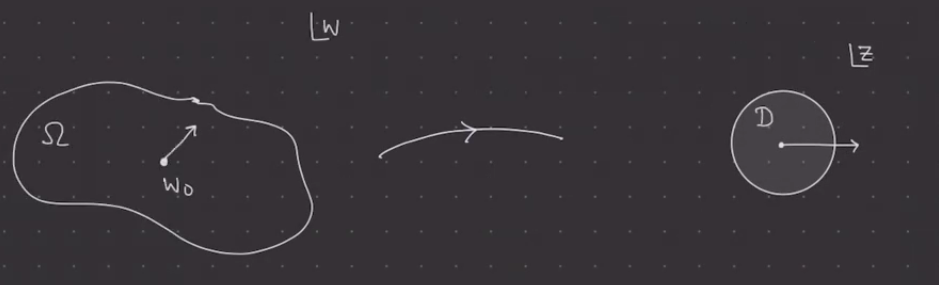
\includegraphics[width=0.7\linewidth]{3}
	\caption{}
	\label{fig:3}
\end{figure}
Let us imagine we are solving the following electrostatics problem:
\begin{equation}
\nabla^2\phi =-\delta(x)\delta(y)
\end{equation}
the potential in two dimensions behaves as
\begin{equation}
\phi\sim -\frac{1}{2\pi}\log r,~~~~~~r=\sqrt{x^2+y^2}
\end{equation}
We can map this to
\begin{equation}
	\Phi= -\frac{1}{2\pi}\log z
\end{equation}
The electrostatic potential with unit charge at $w_0$ and vanishing potential the boundary. From  $\phi$ in this domain we can construct $\Phi(w)$. Physically the situation is like punching a hole in a 2d conductor and placing a charge.
\begin{equation}
\Phi(w)=-\frac{1}{2\pi}\log (ze^{i\alpha})
\end{equation} 
is a conformal map from $w\to z$ plane which preserves the physical solution of the problem. Fixing $\alpha$, fixes a direction.\\\\
\begin{equation}
w=f(z)
\end{equation}
mapos the domain $\Omega$ to $D$. To get the inverse map $z=f^{-1}(w)$ we demand $f'(z)\neq 0$. IF
\begin{equation}
f=u+iv
\end{equation}
Then $\nabla^2u=\nabla^2 v=0$ and $u$ can be viewed as a solution to 3 dimensional Laplace equations if we have cylindrical symmetry. Let us use this to understand some problems we have already seen before.\\\\
Take $\phi=u= \Re f$ as the electrostatic potential, lines of constant $u$ gives equipotential. $v$ is field lines.\\\\
\underline{Example}
Uniform charge density wire along $z=x_3$. The equipotentials are circles and field lines go straight out.
\begin{figure}[H]
	\centering
	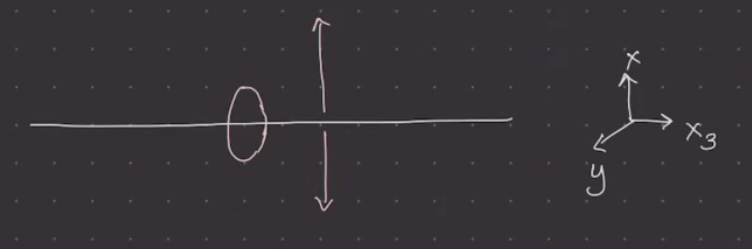
\includegraphics[width=0.7\linewidth]{4}
	\caption{}
	\label{fig:4}
\end{figure}
We have
\begin{equation}
\begin{aligned}
\Phi&=2\lambda \log z\\
\phi&=2\lambda \log r
\end{aligned}
\end{equation}
The equipotentials are $\Re[\Phi]=constant$ give circles in $x,y$ plane. Field lines come from $\Im(\phi)=2\lambda \Theta$.
\\\\
\underline{Example II}
\\\\
Two semi-infinite capacitor places at $y={\pi,-\pi}$ and hold them at constant potential $V(y=\pm \pi)=\pm \pi$. Sketching this, we now the equipotentials just go along the direction of the plates. We can use the exponential map to open it up to (almost) the whole complex plane, so taking $z\to1+z+e^z$. This maps a strip and maps it to the complex plane with two cuts. We can then solve the Laplace equation in the complex plane, i.e. we just get a linear function and the B.C.'s force the solutions to be non-zero.\\\\
The exponential map takes the complex plane and wraps it into a cylinder.
\begin{figure}[H]
	\centering
	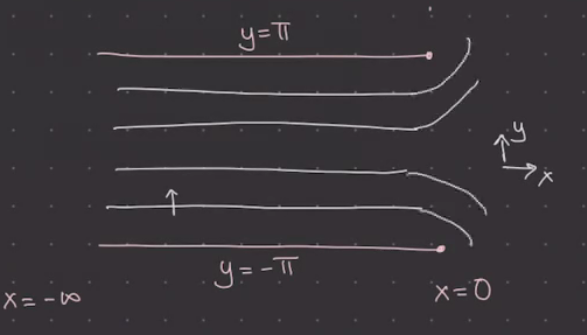
\includegraphics[width=0.7\linewidth]{5}
	\caption{}
	\label{fig:4}
\end{figure}
%\underline{Example III}
%\\\\
%Two cylinders held at potentials $u$ and $v$ of equal size:
%\begin{figure}[H]
%	\centering
%	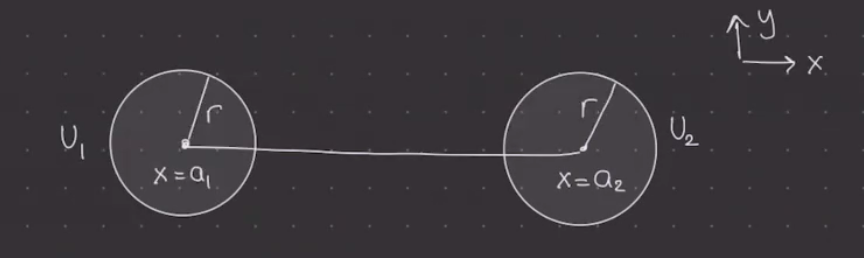
\includegraphics[width=0.7\linewidth]{6}
%	\caption{}
%	\label{fig:4}
%\end{figure}
%We want to find
\newpage
\section*{Homework 1}
\section*{Problem 1}
\subsection*{Part a}
We compute
\begin{equation}
\oint_{|z|=3} \dd z\frac{4z-3}{z(z-2)}
\end{equation}
Inside the contour this has poles at $z=0$ and $z=2$ so using 
\begin{equation}
	\oint _C \dd z  f(z)=2\pi i \sum_{a_i\in D}\Res[f(a_i)]
\end{equation}
We get
\begin{equation}
\begin{aligned}
	\oint_{|z|=3} \dd z\frac{4z-3}{z(z-2)}=&2\pi i \left\{\Res[\frac{4z-3}{z(z-2)}]_{z=0}+\Res[\frac{4z-3}{z(z-2)}]_{z=2}\right\}\\
	=&2\pi i \left\{\frac{4\times 0-3}{(0-2)}+\frac{4\times 2-3}{2}\right\}\\
	=&2\pi i \left\{\frac{3}{2}+\frac{5}{2}\right\}\\	
	=&8\pi i 
\end{aligned}
\end{equation}
\subsection*{Part b}
Similarly
\begin{equation}
	\begin{aligned}
		\oint_{|z|=3} \dd z\frac{e^z}{(z-1)(z-2)}=&2\pi i \left\{\Res[\frac{e^z}{(z-1)(z-2)}]_{z=1}+\Res[\frac{e^z}{(z-1)(z-2)}]_{z=2}\right\}\\
		=&2\pi i \left\{-e+e^2\right\}\\
	\end{aligned}
\end{equation}
\section{Problem 2}
\subsection*{Part a}
Computing
\begin{equation}
	\begin{aligned}
		\int_{0}^{\infty}\dd x\frac{2x^2-1}{x^6+1}
		=&	\frac{1}{2}\int_{-\infty}^{\infty}\dd x\frac{2x^2-1}{x^6+1}
		\\
		=&\frac{1}{2}\oint_{|z|=2} \dd z\frac{2z^2-1}{z^6+1}\\
		=&\pi i \left\{\Res[\frac{2z^2-1}{z^6+1}]_{z=i}+\Res[\frac{2z^2-1}{z^6+1}]_{z=(-1)^{\frac{1}{6}}}+\Res[\frac{2z^2-1}{z^6+1}]_{z=(-1)^{\frac{5}{6}}}\right\}\\
		=&\pi i \left\{\frac{i}{2}+\frac{1}{6}\left(-2i+(-1)^{\frac{1}{6}}\right)+\frac{1}{6}\left(-2i+(-1)^{\frac{5}{6}}\right)\right\}\\
		&=0
	\end{aligned}
\end{equation}
\subsection*{Part b}
For this integral we will be using $\sin n\theta =\frac{1}{2i}\left(z^n-z^{-n}\right)$, $\cos n\theta =\frac{1}{2}\left(z^n+z^{-n}\right)$ and $\dd \theta=\frac{1}{iz}\dd z$. Computing
\begin{equation}
	\begin{aligned}
		\int_{0}^{\pi}\dd x\frac{\cos^2(3x)}{5-4\cos(2x)}
		=&\oint_{|z|=1}\frac{\dd z}{iz}\frac{\left(z^3+\frac{1}{z^3}\right)^2}{4 \left(1-2 \left(z^2+\frac{1}{z^2}\right)\right)}\\
		=&\oint_{|z|=1}\dd z \frac{i \left(z^6+1\right)^2}{8 z^9-4 z^7+8 z^5}\\
			=&2\pi i \left\{
			\Res[\frac{\left(z^6+1\right)^2}{8 z^9-4 z^7+8 z^5}]_{z=0}
			\right\}\\
			=&\frac{3\pi}{16}
	\end{aligned}
\end{equation}
\subsection*{Part c}
The following integral is a little trickier. First we rewrite the outer cosine at the real part of a complex function and combine the exponentials
\begin{equation}
\begin{aligned}
\int_{0}^{\pi}\dd x\, e^{\cos(x)}\cos[nx-i\sin(x)]&=\frac{1}{2}\Re\left[\int_{-\pi}^{\pi}\dd x\, e^{\cos(x)+inx-i\sin(x)}\right]\\
&=\frac{1}{2}\Re\left[\int_{-\pi}^{\pi}\dd x\, e^{inx}e^{e^{-ix}}\right]
\end{aligned}
\end{equation}
where we have used $e^{-ix}=\cos(x)-i\sin(x)$. Now
substituting $z=e^{-ix}$, which leads to $\dd z=-i e^{-ix} \dd x=-iz \dd x$
%%%%%%%%%%%%%%%%%%%%%%%%%%%%%%%%%%%%%%%%%%%%%%%%%%%%
\begin{equation}
	\begin{aligned}
\int_{0}^{\pi}\dd x\, e^{\cos(x)}\cos[nx-\sin(x)]&=\frac{1}{2}\Re\left[\int_{-\pi}^{\pi}\dd z\, \frac{e^{z}}{z^{(n+1)}}\right]\\
&=\frac{1}{2}\Re\left[\oint_{|z|=1}-i\dd z\, \frac{e^{z}}{z^{(n+1)}}\right]\\
	\end{aligned}
\end{equation}
This has an $n$'th order pole at $z=0$. We can find the residues using
\begin{equation}
	\Res[f(z=a)]=\frac{1}{(m-1)!}\lim_{z\to a}\dv[m-1]{}{z}[(z-a)^mf(z)]
\end{equation}
which in this case is particularly easy since we have an exponential function, so
\begin{equation}
	\begin{aligned}
		\int_{0}^{\pi}\dd x\, e^{\cos(x)}\cos[nx-\sin(x)]&=
		\Re\left [\pi \Res[\frac{e^{z}}{z^{(n+1)}}]_{z=0}\right]\\
		&=\frac{\pi}{n!}
	\end{aligned}
\end{equation}
\subsection*{Part d and Part e}
Lastly we have the two $\sinh$ integrals, with different contours. Let us first note that we have the Laurent series:
\begin{equation}
\frac{1}{\sinh z}=\frac{1}{z}-\frac{1}{6}z^2+\frac{7}{16}z^3+\cdots
\end{equation}
so that the combination
\begin{equation} \label{eq:sinh}
	\frac{1}{z^2\sinh z}=\frac{1}{z^3}-\frac{1}{6z}+\frac{7}{16}z+\cdots
\end{equation}
Further, we know that the zeroes of $\sinh z$ are at $n\pi i $, $n\in\mathds{Z}$ while for $z^2$ it is at $0$. This means that we for the contour $|z|=1$ only have to take the residue at $z=0$, while for $|z|=4$ also have to include the residue at $z=i\pi$. \eqref{eq:sinh} has a third order pole and a first order pole however since calculating the residue of the third order pole requires differentiating twice it's residue is just zero and we only need the contribution from the first order pole
\begin{equation}
\begin{aligned}
\oint_{|z|=1}\dd z\,\frac{1}{z^2\sinh z}  &=2\pi i \Res[\frac{1}{z^2\sinh z}]_{z=0}\\
&=2\pi i \left[-\frac{1}{6}\right]\\
&=-\frac{\pi i}{3}
\end{aligned}
\end{equation}
For the larger contour we, as mentioned, have to include the residue at $i\pi$ and $-i\pi$. The residue at this point be calculated using
\begin{equation}
\Res[\frac{p(z)}{q(z)}]_{z=a}=\lim_{z\to a}\left[\frac{p(z)}{q'(z)}\right]
\end{equation}
where $q(z)$ has a pole at $z=a$ and $p(z)$ does not. Hence taking $q(z)=\sinh(z)$ and $p(z)=z^2$  we have
\begin{equation}
\begin{aligned}
\Res[\frac{1}{z^2}\frac{1}{\sinh}]_{z=i \pi}&=\lim_{z\to i\pi }\left[\frac{1}{z^2}\frac{1}{\cosh}\right]\\
&=\frac{1}{\pi^2}
\end{aligned}
\end{equation}
and
\begin{equation}
	\begin{aligned}
		\Res[\frac{1}{z^2}\frac{1}{\sinh}]_{z=-i \pi}&=\lim_{z\to -i\pi }\left[\frac{1}{z^2}\frac{1}{\cosh}\right]\\
		&=\frac{1}{\pi^2}
	\end{aligned}
\end{equation}
So the total contour integral is
\begin{equation}
	\begin{aligned}
		\oint_{|z|=4}\dd z\,\frac{1}{z^2\sinh z}  &=2\pi i \left\{
		\Res[\frac{1}{z^2\sinh z}]_{z=0}+\Res[\frac{1}{z^2\sinh z}]_{z=i\pi}+\Res[\frac{1}{z^2\sinh z}]_{z=-i\pi}
		\right\}\\
		&=2\pi i \left[-\frac{1}{6}+\frac{1}{\pi^2}+\frac{1}{\pi^2}\right]\\
		&=2\pi i \left[-\frac{1}{6}+\frac{2}{\pi^2}\right]
	\end{aligned}
\end{equation}
\section*{Problem 3}
Using Causchy's integral formula
\begin{equation}
	\begin{aligned}
f(a)&=\frac{1}{2\pi i}\oint_{z=|R|} \dd z\,\frac{f(z)}{z-a}
	\end{aligned}
\end{equation}
We can subtract the following term since it is zero inside this contour by Cauchy's theorem
\begin{equation}
	\begin{aligned}
		0&=\frac{1}{2\pi i}\oint_{z=|R|} \dd z\,\frac{f(z)\bar a}{ R^2-\bar az}
	\end{aligned}
\end{equation}
So we get
\begin{equation}
	\begin{aligned}
		f(a)&=\frac{1}{2\pi i}\oint_{z=|R|} \dd z\,\left[\frac{f(z)}{z-a}-\frac{f(z)\bar a}{ R^2-\bar az}\right]\\
		&=\frac{1}{2\pi i}\oint_{z=|R|} \dd z\,f(z)\frac{R^2-\bar a a}{(z-a)(R^2-\bar az)}\\
	\end{aligned}
\end{equation}
Where we have put everything on a common denominator in the last term. Expanding this denominator and writing $|a|^2=\bar a a$ we find
\begin{equation}
	\begin{aligned}
		f(a)
		&=\frac{1}{2\pi i}\oint_{z=|R|} \frac{\dd z}{z}\,f(z)\frac{R^2-|a|^2}{R^2-2\Re(a\bar z)+|a|^2}
	\end{aligned}
\end{equation}
Then letting $a=re^{i\theta}$ and integrating around the contour by setting $z=Re^{i\phi}$, $0\leq \phi \leq 2\pi$ \footnote{Note that we in the above have used $\bar z=z^{-1}$}. Further we have $\dd z=iRe^{i\phi}\dd \phi=iz\dd \phi$ and $|a|^2=r^2$, then
\begin{equation}
	\begin{aligned}
f(re^{i\theta})&=\frac{1}{2\pi i}\int_{0}^{2\pi} \dd \phi\,f(Re^{i\phi})\frac{R^2-r^2}{R^2-2Rr\cos(\theta-\phi)+r^2}
	\end{aligned}
\end{equation}
\section*{Problem 4}
\subsection*{Part a}
We have the Navier-Stokes equation:
\begin{equation}
\partial_t \bm u+\bm u\cdot  \nabla\bm u=-\nabla \left(\frac{1}{\rho} p- V\right)+\nu\nabla^2 \bm u
\end{equation}
Taking the curl on both sides we use the fact that the curl of a gradient of scalar is zero 
\begin{equation} \label{eq:ns}
	\partial_t \bm \omega+\nabla\times(\bm u \cdot \nabla\bm u)=+\nu\nabla^2 \bm w
\end{equation}
Furtherm, since $\nu=0$ in this case
\begin{equation} \label{eq:ns}
	\partial_t \bm \omega+\nabla\times(\bm u \cdot \nabla\bm u)=0
\end{equation}
Then using the fact that
\begin{equation}
\bm u \cdot \nabla\bm u=\frac{1}{2}\nabla u^2-\bm u\times (\nabla \times \bm u)=\frac{1}{2}\nabla u^2-\bm u\times \bm \omega
\end{equation}
we can rewrite
\begin{equation}
\begin{aligned}
\nabla\times(\bm u \cdot \nabla\bm u)&=\frac{1}{2}\nabla\times\nabla u^2-\nabla\times (\bm u\times \bm \omega)\\
&=\nabla\times (\bm \omega \times \bm u)\\
&=(\bm u \cdot \nabla)\bm\omega -(\bm \omega  \cdot \nabla)\bm u +\bm\omega (\nabla\cdot \bm u)+\bm u (\nabla\cdot \bm \omega )\\
&=(\bm u \cdot \nabla)\bm\omega -(\bm \omega  \cdot \nabla)\bm u
\end{aligned}
\end{equation}
where the we have used $\nabla\cdot \bm u=0$ and $\bm u(\nabla \cdot \bm \omega)=\bm u(\nabla \cdot (\nabla \times \bm u))=0$ in the third line. Inserting this back into \ref{eq:ns}:
\begin{equation} \label{eq:ns2}
	\partial_t \bm \omega+(\bm u \cdot \nabla)\bm\omega =(\bm \omega  \cdot \nabla)\bm u
\end{equation}
Or in index notation:
\begin{equation} \label{eq:ns2}
	\partial_t \omega_i+ u ^j \partial_j\omega_i = \omega^j  \partial_j u_i
\end{equation}
\subsection{Part b}
If $\bm \omega =\nabla\times \bm u =0$, we could write
\begin{equation}
\bm u=\nabla \phi
\end{equation}
Since the equation
\begin{equation}
\nabla\times \nabla\phi =0
\end{equation}
is automatically satisfied. This is similar to the gauge potential in electrodynamics. Further from the incompressibility we know $\phi$ satisfies the Laplace equation
\begin{equation}
\nabla\cdot u=\nabla^2 \phi=0
\end{equation}
\subsection*{Part c}
\begin{equation}
	\nabla \partial_t \phi+\frac{1}{2}\nabla u^2=-\nabla \left(\frac{1}{\rho} p+ V\right)
\end{equation}
\begin{equation}
	\nabla \left(\partial_t \phi+\frac{1}{2} u^2+\frac{p}{\rho} + V\right)=0
\end{equation}
\begin{equation}
 \left(\partial_t \phi+\frac{1}{2} u^2+\frac{p}{\rho} + V\right)=F(t)
\end{equation}
\begin{equation} \label{eq:flow}
	\left(\partial_t \phi+\frac{1}{2} u^2+\frac{p}{\rho} + V\right)=F(t)
\end{equation}
\subsection*{Part d}
We have already shown that since we have irrotational flow, i.e. $\nabla\times \bm u=0$ we can write the flow field as a gradient
\begin{equation}
\begin{aligned}
	v_x&=\partial_x \phi\\
	v_y&=\partial_y \phi
\end{aligned}
\end{equation}
Further, since we have an in-compressible fluid, i.e. $\nabla\cdot u=0$ we can write it as a "curl" of a scalar\footnote{Since there doesn't exist such thing as a curl of scalar function, the use of curl in this case should be taken as meaning \begin{equation}
\bm v=\nabla\times \begin{pmatrix}
1\\1
\end{pmatrix}\chi
\end{equation}}
\begin{equation}
\begin{aligned}
v_x&=\partial_y \chi\\
v_y&=-\partial_x \chi
\end{aligned}
\end{equation}
since it automatically satisfies $\nabla\cdot u=0$. We see that in this case we can use either $\phi$ or $\chi$ to solve \eqref{eq:flow} and that further
\begin{equation}
	\begin{aligned}
		\partial_x \phi&=\partial_y \chi\\
		\partial_y \phi&=-\partial_x \chi
	\end{aligned}
\end{equation}
These are just the Cauchy-Riemann relations and so we we can construct an analytic function out of these, known as the stream function
\begin{equation}
\Phi=\phi+i\chi
\end{equation}
This stream-function also solves \eqref{eq:flow} since the derivatives act linearly on it as a consequence of the Cauchy-Riemann relations implying $(\nabla\phi)\cdot (\nabla\chi)=0$
\begin{equation}
(\nabla \Phi)^2=(\nabla \phi+i\nabla\chi)(\nabla \phi-i\nabla\chi)=(\nabla\phi)^2+(\nabla\chi)^2
\end{equation}
\subsection{Part e}
Milne–Thomson theorem
\begin{equation}
\tilde \Phi= \Phi(z)+\bar \Phi(\frac{a^2}{z})
\end{equation}
restricting to $z<1$
%%%%%%%%%%%%%%%%%%%%%%%%%%%%%%%%%%%%%%%%%%%%%%%%%%
\end{document}
